
\begin{center}
$TopLeftMin(r, (x, y))$ = $min _{a_1 \leq i \leq x, a_2 \leq j \leq y}$ $A(i,j)$; 

$TopRightMin(r, (x, y))$ = $min _{a_1 \leq i \leq x, y \leq j \leq b_2}$ $A(i,j)$; 

$BottomLeftMin(r, (x, y))$ = $min _{x \leq i \leq b_1, a_2 \leq j \leq y}$ $A(i,j)$; 

$TopRightMin(r, (x, y))$ = $min _{x \leq i \leq b_1, y \leq j \leq b_2}$ $A(i,j)$; \\
\end{center}

A straightforward implementation of \emph{DominanceMin} structures costs $\mathcal{O}(N \log^2 N)$ comparisons. To reduce the number of comparisons to linear, we first sort canonical ranges in the increasing order of their sizes. Constructing \emph{DominanceMin} for size 1 is trivial and does not require any comparison. For size greater than 1, two smaller \emph{DominanceMin} structures can be merged to obtain a new \emph{DominanceMin}. For a range $r$ = $I_1 \times I_2$, the number of comparisons to construct \emph{DominanceMin} is at most $4 |I_2| \log |I_1|$ when $|I_1| \geq |I_2|$ or  $4 |I_1| \log |I_2|$ when $|I_2| > |I_1|$. Below is demonstrated an algorithm for computing \emph{TopLeftMin($r,(x,y)$)} when $|I_1| \geq |I_2|$.\\
Let $I_1=[a_1,b_1]$, $I_2=[a_2,b_2]$. $I_1$ is split into two intervals $I_3$=$[a_1, (a_1+b_1-1)/2]$ and $I_4$=$[(a_1+b_1+1)/2,b_1]$. The \emph{TopLeftMin} structures from smaller canonical ranges $r_1$ =$I_3 \times I_2$ and $r_2$=$I_4 \times I_2$ are combined as follows:
\begin{enumerate}
\item For any index $(x,y)$ $\in$ $r_1$, \emph{TopLeftMin}($r, (x, y)$) = \emph{TopLeftMin}($r_1, (x, y)$)
\item For index  $(x,y) \in r_2$, and  $s = TopLeftMin(r_1, (a_1+b_1-1)/2,y))$. Since the second part \emph{TopLeftMin}($r_2, (x, y)$ for $x$ $\in$ $I_4$ is non-increasing and we can do a binary search of $s$ in that sequence and compute \emph{TopLeftMin}($r, (x, y)$) for $x$ $\in$ $I_4$. This requires at most $\left \lceil\log_2 (|I_4|+1) \right \rceil \leq \log_{2}I_4+1=log_2|I_1|$ comparisons. For each $y$ $\in$ $I_2$, we do the above binary search to compute \emph{TopLeftMin}($r, (x, y)$) for $x \in I_4$. Hence the total number of comparisons made is $|I_2| \log |I_1|$. To build all the 4 \emph{DominanceMin} structure it will take $4 |I_2| \log |I_1|$.
\end{enumerate}

\begin{theorem}[Preprocessing Complexity]
The proposed 2D RMQ preprocessing algortihm uses $\mathcal{O}(N)$ comparisons. 
\end{theorem}
For each $0 \leq i \leq \log m$ and $0 \leq j \leq \log n$, let $F(i, j)$ be the set of $2^i$ by $2^j$ canonical intervals. If $i \geq j$, then the comparisons made for constructing all canonical ranges is $\mathcal{O}(|F(i, j)|.2^j \log 2^i)=\mathcal{O}(\frac{i}{2^i}.N)$. The number of comparisons made for constructing $\cup _{i \geq j} F(i, j)$ is in the order of 
\begin{center}
$\sum \limits_{i=0}^{\log m} \sum \limits_{j=0}^{i} \frac{i}{2^i}N=(\sum \limits_{i=0}^{\log m} \frac{i(i+1)}{2^i})N$ \\
$\leq (\sum \limits_{i=0}^{\infty} \frac{i(i+1)}{2^i})N = O(N)$
\end{center}
Similarly, $\cup _{i \geq j} F(i, j)$ is also constructed in $\mathcal{O}(N)$ comparisons. Hence $\mathcal{O}(N)$ comparisons are made for constructing \emph{DominanceMin} structures for \emph{CR}.

%\begin{figure}[H]%
%    \centering
%    {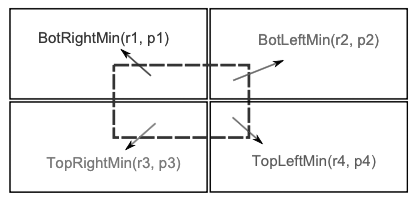
\includegraphics[height=3cm,]{img/yuan2d.png} }
%    \caption{4 \emph{DominanceMin} structure for querying 2D \emph{RMQ}}%
%    \label{fig:yuan2d}%
%\end{figure}

\section{2D RMQ: Querying}
\begin{center}
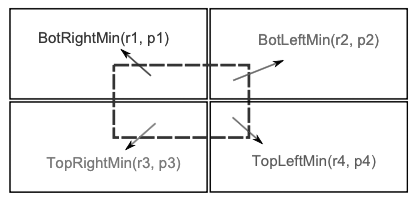
\includegraphics[height=3cm,]{img/yuan2d.png}

\end{center}

For any query range $q$, we can always divide it into 4 parts or canonical ranges, which are all pre-computed and each subquery is a 2-side range query with some canonical range. The above figure shows how the query is splitted into 4 canonical ranges \emph{BotRightMin}, \emph{BotLeftMin},\emph{TopLeftMin},\emph{TopRightMin} respectively.
Hence the final result can be obtained with at most 3 comparisons. However to find this canonical ranges in constant time, Yuan et al. defines the faster approach same as 1D where auxiliary tree for $CIS_1$ and $CIS_2$ are built in linear space and time. \\
\begin{theorem}[Querying Complexity]
With the linear-comparison preprocessing for a 2D array, it takes at most 3 comparisons to answer a range minimum query.
\end{theorem}